\section{Introduction}

Trust plays an integral part in network communications.
It effectively determines from whom and from which services or applications, users accept information or are willing to send information.
When a new device attempts to integrate itself into a new environment for the first time, it must go through a verification process that identifies the device to be legitimate.
Bootstrapping is the onboarding process through which an entity learns the presence of other entities in the network along with learning of the other entity’s current state.
It is the process that prevents the infiltration of malicious nodes into the network and helps in making sure that legitimate devices or entities are getting the necessary accesses or privileges.
Trust bootstrapping thus assists the requester in making the right choice of services

\begin{figure}[h]
\centering
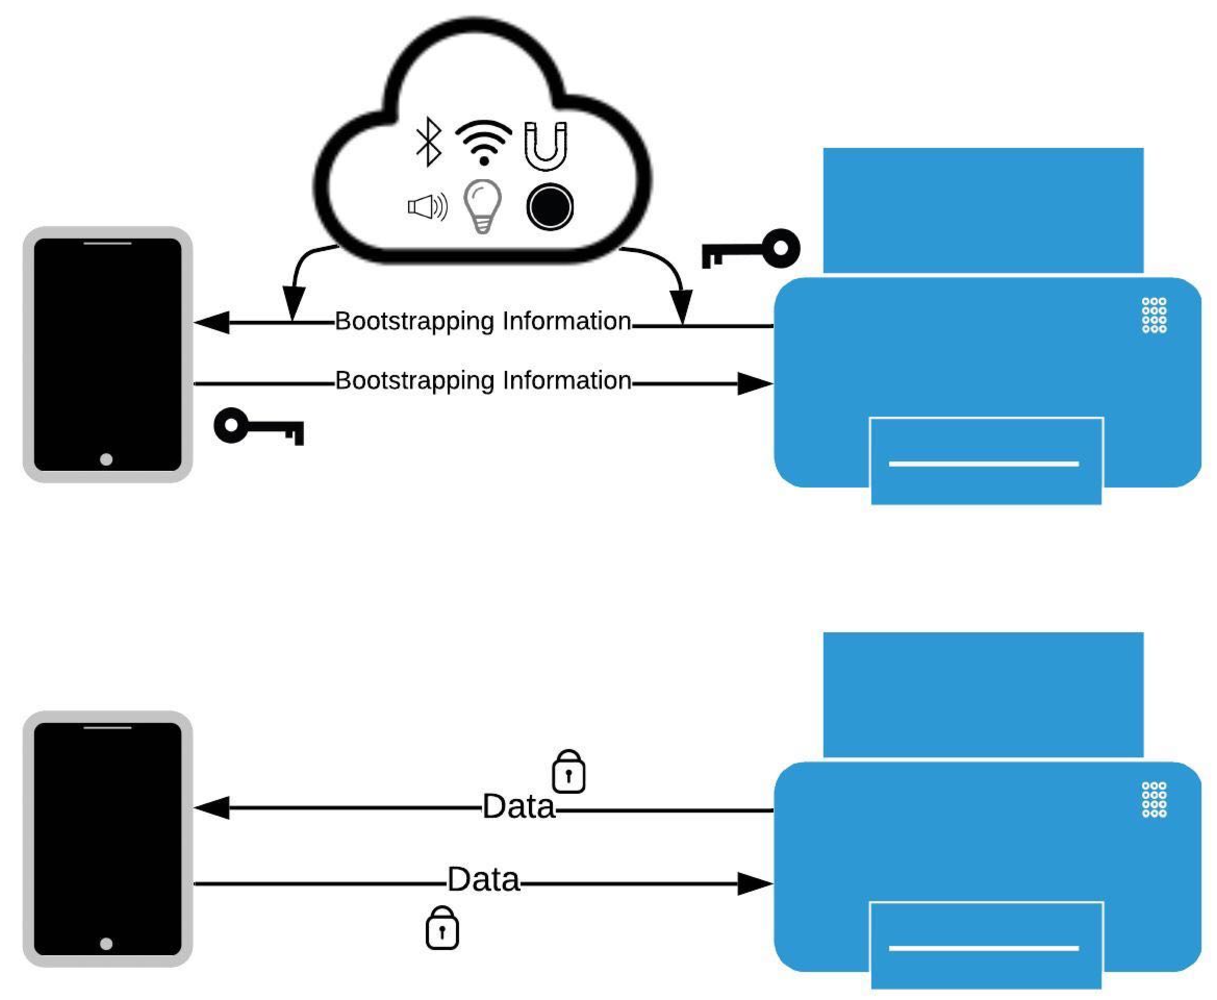
\includegraphics[scale=0.5]{figures/picture.pdf}
\caption{General Bootstrapping Process}
  \label{fig:pic}
\end{figure}
